\section{Theoretical Basis}
\subsection{Bézier Curve}
Bezier curves is a set of locally generated points that can be constructed and positioned from a set of control points.
The more local control points being constructed, the smoother curve becomes.
Bezier curves are widely used in real life for tasks requiring smooth and precise shapes.
They are essential in graphic design and digital art for creating scalable vector graphics and smooth font outlines.

\subsubsection{Linear Interpolation}

\begin{wrapfigure}{H}{0.4\textwidth}
  \centering
  \addtolength{\belowcaptionskip}{-4.0ex}
  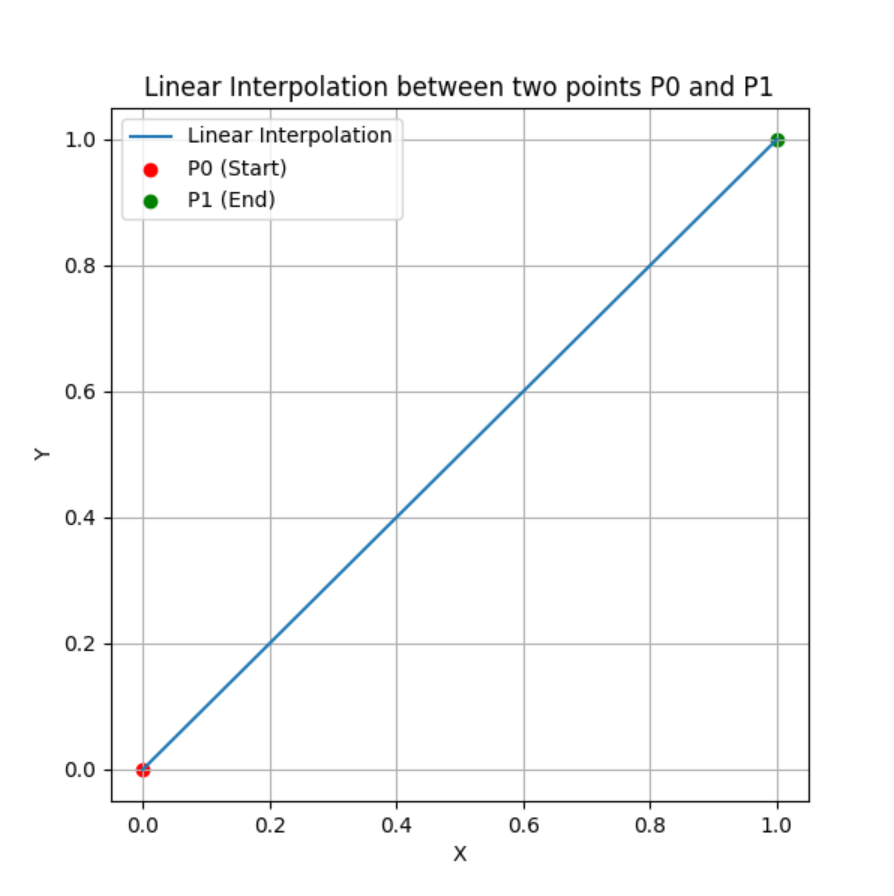
\includegraphics[width=0.4\textwidth]{single_lerp.png}
  \caption{Linear Interpolation}
\end{wrapfigure}
By definition of the Bezier Curve, Linear Interpolation is the main foundation of constructing the points on the curve.
This is a method of estimating an intermediate value between two points $P_0$ and $P_1$, based on a parameter t that runs on the interval $[0;1]$.
$$P(t)=(1-t)P_0+tP_1$$
where t=0 gives $P_0$ and t=1 gives $P_1$.

\subsubsection{General Form of Bézier Curves}
In order to construct a curve, multiple Linear Interpolations can be performed nested inside each other.
For example, interpolating $P_3$ between $P_0$ and $P_1$, $P_4$ between $P_1$ and $P_2$ and then do the same with $P_5$ between $P_3$ and $P_4$ will give us a quadratic Bezier Curve.
In this case, $P_0$, $P_1$ and $P_2$ are called "control points".
The general form of a Bézier curve allows it to be extended to any degree $n$ based on the number of control points $P_0, P_1, \ldots, P_n$. The curve is defined as:
$$B(t) = \sum_{i=0}^{n} \binom{n}{i} (1 - t)^{n-i} t^i P_i$$
Where:
\begin{itemize}
  \item $B(t)$ is the point on the Bézier curve at parameter $t \in [0, 1]$,
  \item $\binom{n}{i} = \frac{n!}{i!(n-i)!}$ is the binomial coefficient,
  \item $P_i$ is the $i^{th}$ control point,
  \item $n$ is the degree of the Bézier curve, ($n+1$) is the number of control points.
\end{itemize}
\begin{figure}[h]
  \centering
  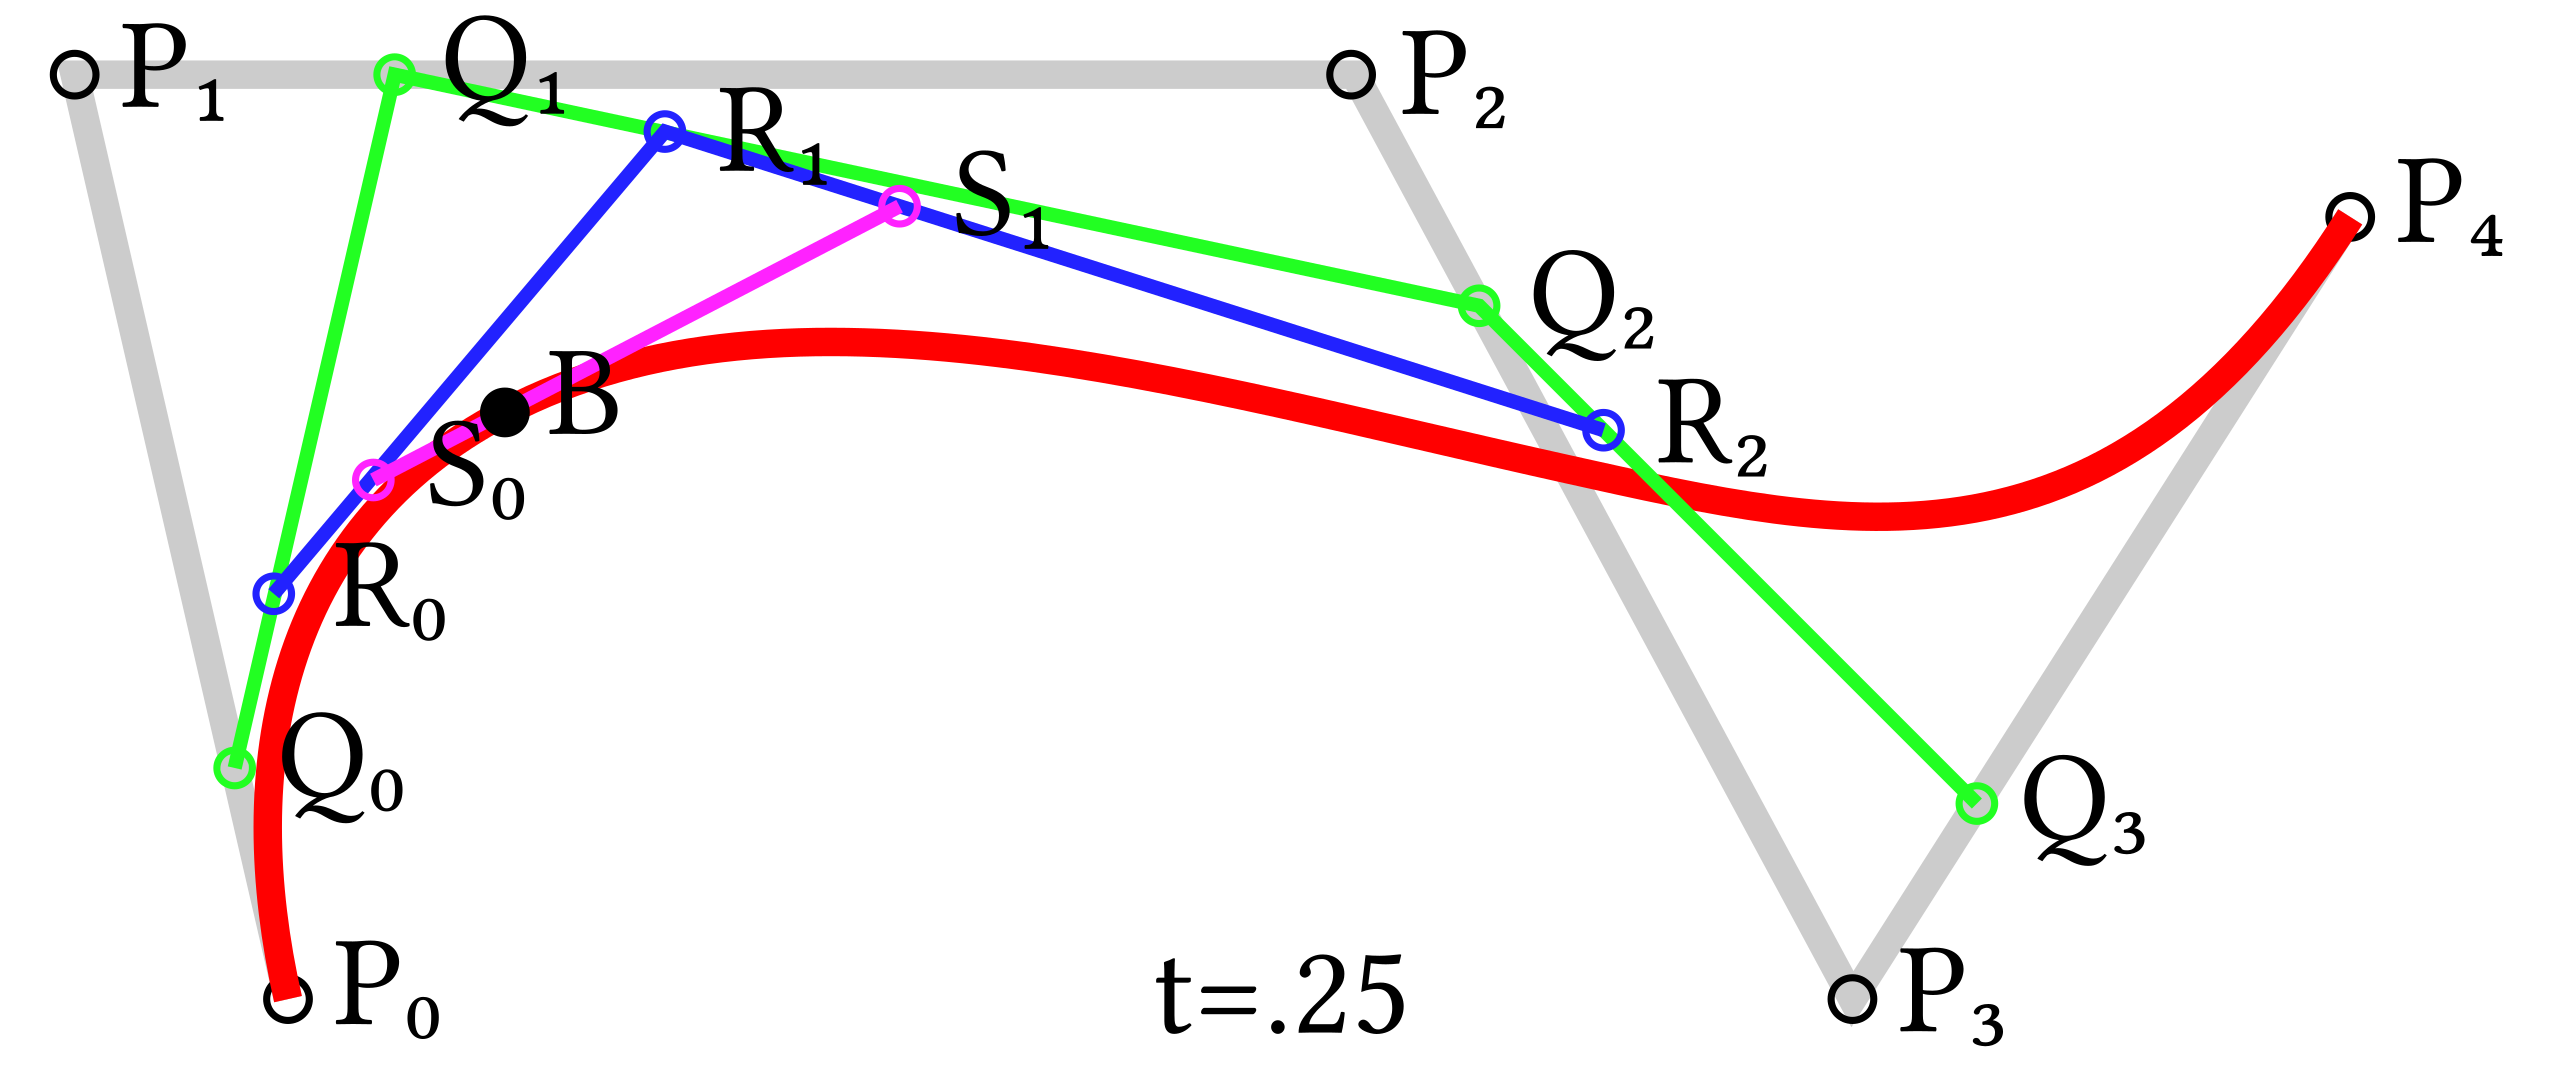
\includegraphics[width=0.45\textwidth]{general_bezier.png}
  \caption{General Form of Bézier Curves}
\end{figure}

\subsubsection*{Example}
\begin{itemize}
  \item $n = 1$, the curve is a simple straight line (single Linear Interpolation).
  \item $n = 2$, the curve is a Quadratic Bezier Curve.
  \item $n = 3$, the curve is a Cubic Bezier Curve.
\end{itemize}
\begin{figure}[ht]
  \centering
  \begin{subfigure}[b]{0.45\textwidth}
    \centering
    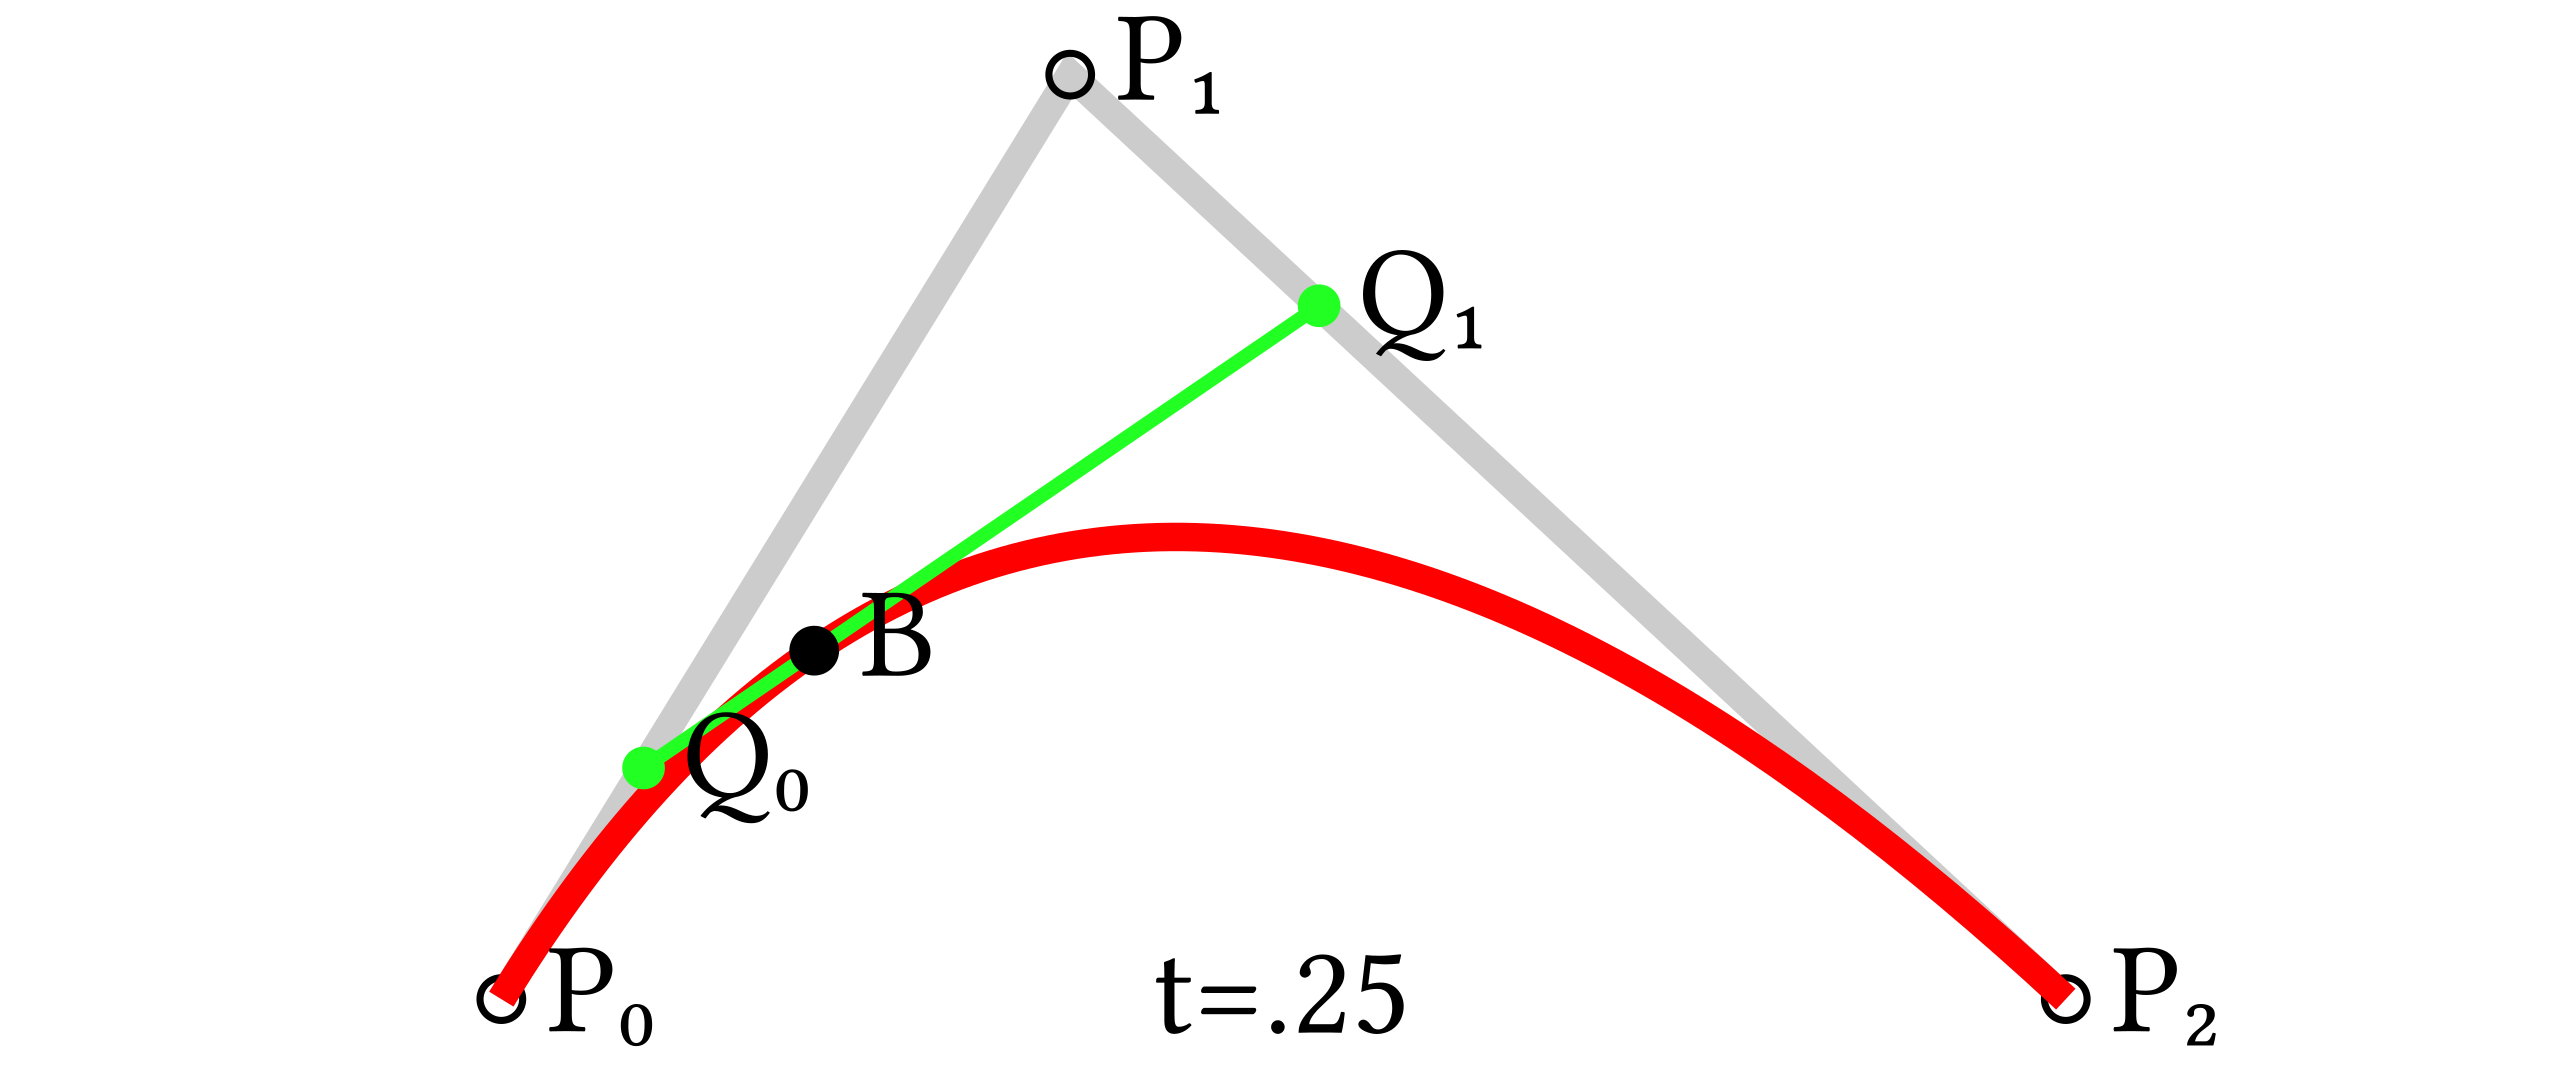
\includegraphics[width=\textwidth]{quadratic_bezier.png}
    \caption{Quadratic Bézier Curve}
  \end{subfigure}
  \hfill
  \begin{subfigure}[b]{0.45\textwidth}
    \centering
    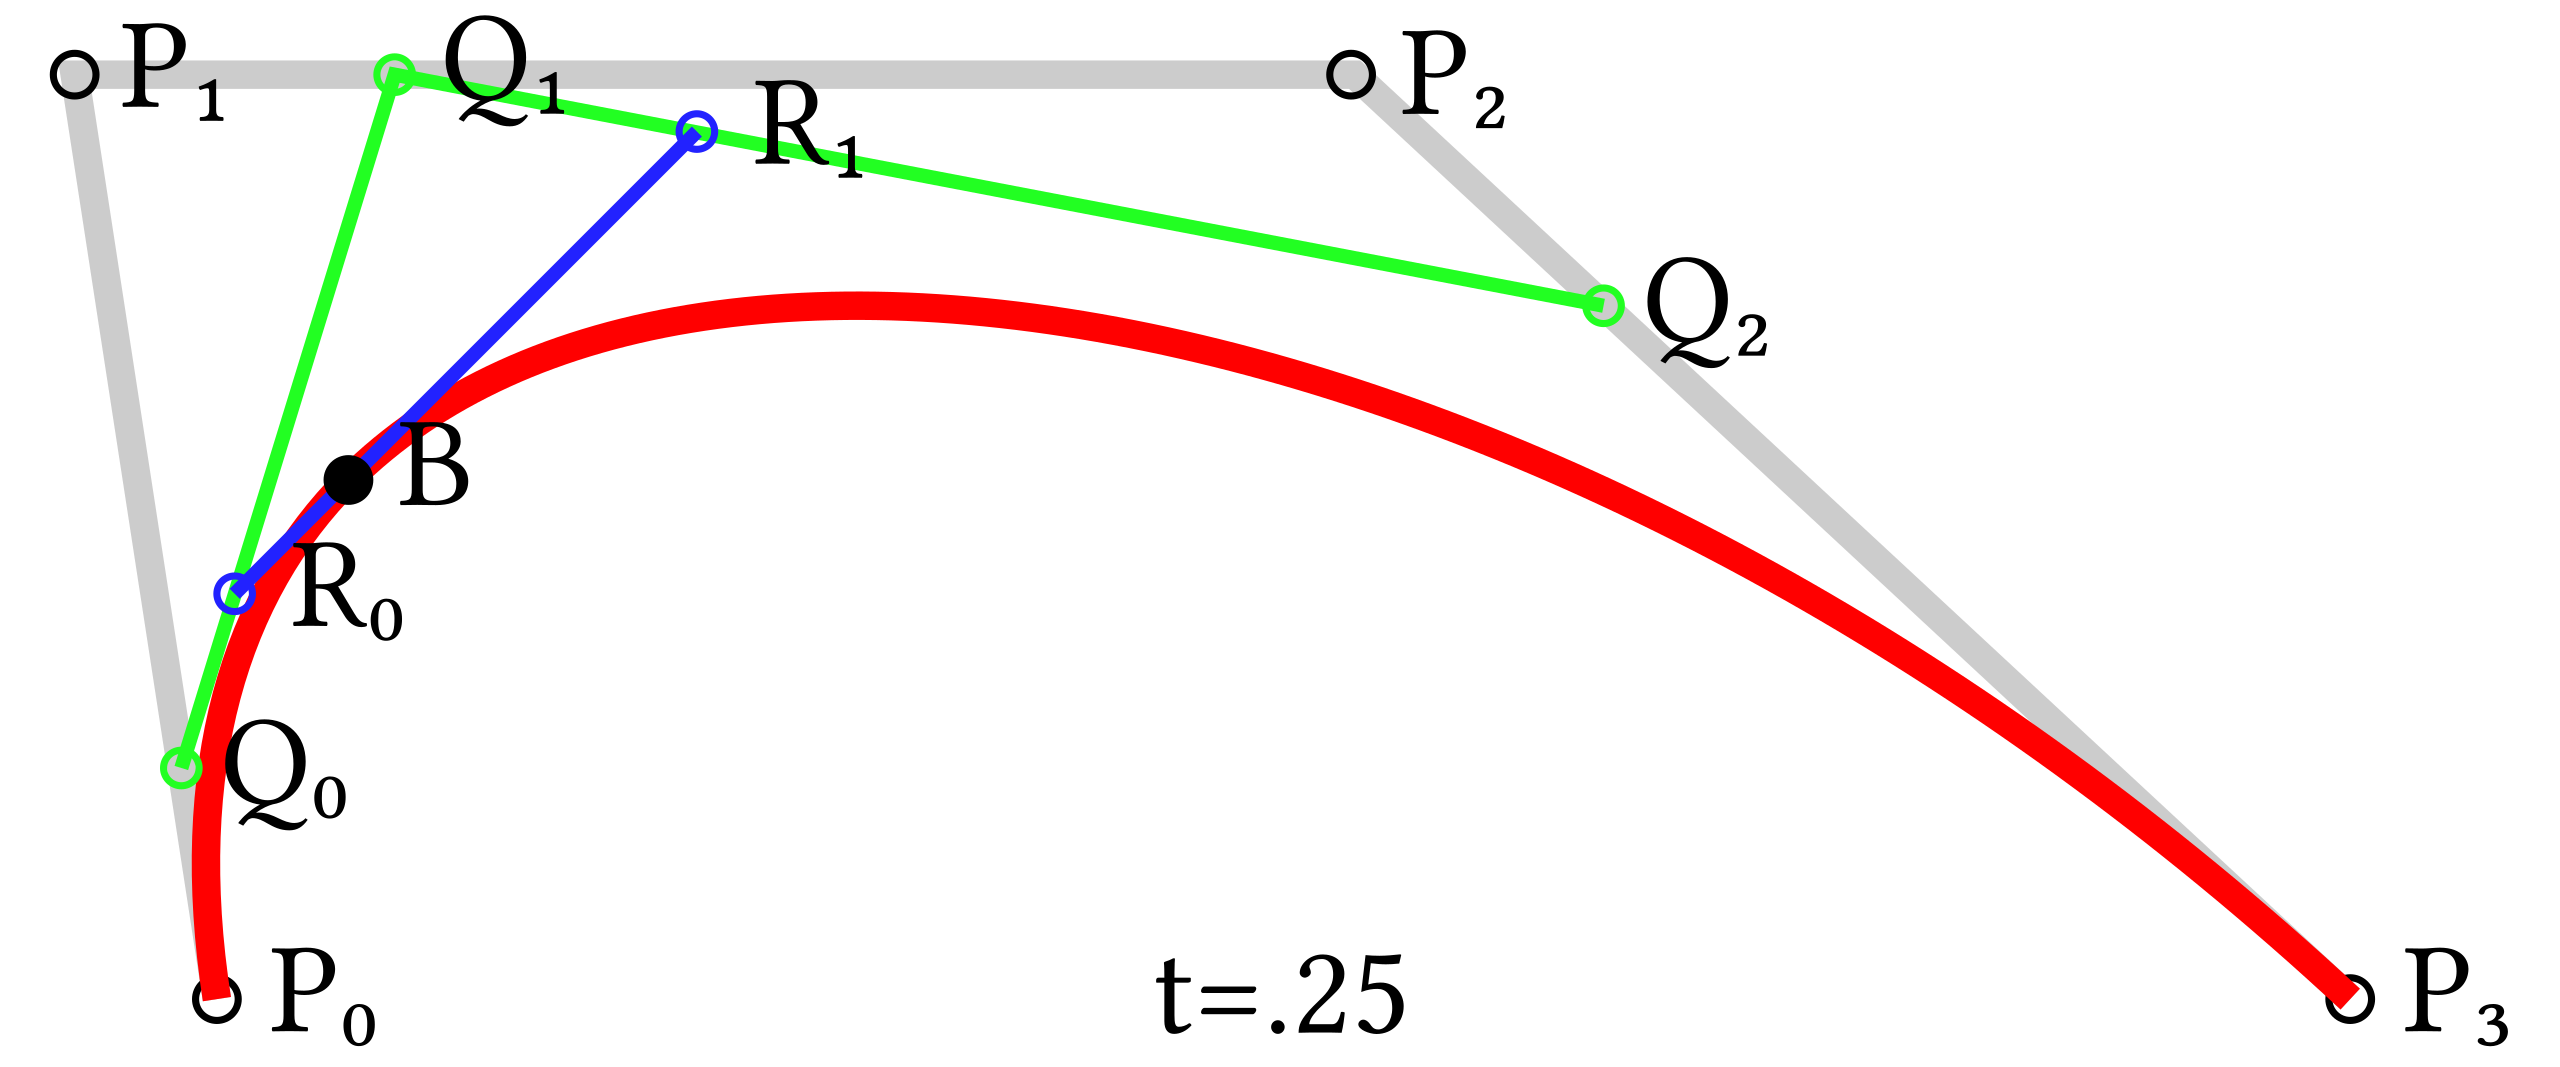
\includegraphics[width=\textwidth]{cubic_bezier.png}
    \caption{Cubic Bézier Curve}
  \end{subfigure}
  \caption{Some cases of Bézier Curve}
\end{figure}

\subsubsection{Properties}
\begin{itemize}
  \item \textbf{Control Points:} The curve starts at $P_0$ and ends at $P_n$. Intermediate control points ($P_1, P_2, \ldots, P_{n-1}$) influence the shape but are not necessarily on the curve.
  \item \textbf{Continuity:} Bézier curves are continuous and smooth, making them ideal for graphics and design applications.
  \item \textbf{Scalability:} Adding more control points increases the degree of the curve, allowing for more complex shapes.
\end{itemize}

% \subsubsection{De Casteljau’s Algorithm}
% De Casteljau's algorithm is a recursive process for constructing Bézier curves. It works by repeatedly blending control points to calculate points on the curve. The steps are as follows:
% \begin{itemize}
%   \item \textbf{Input:} A set of control points $P_0, P_1, \ldots, P_n$ and a parameter $t$ (where $0 \leq t \leq 1$).
%   \item \textbf{Linear Interpolation:}
%     Start with the control points and calculate new points between them using the formula:
%     $$P_{i,j} = (1-t)P_{i-1,j} + tP_{i-1,j+1}$$
%     This finds intermediate points between pairs of control points.
%   \item \textbf{Repeat:}
%     Continue interpolating between the newly created points until only one point remains. This final point lies on the Bézier curve at the parameter $t$.
% \end{itemize}

\subsection{PID Control}
PID is a closed loop algorithm use to help a system achieve a pre-determined setpoint.
For example, PID could be used to adjust the valve of a water pipe to control the water flow inside fixed at a setpoint.
The main formula of PID algorithm is:
$$u(t)=K_I\cdot e(t)+K_P\cdot\int_0^te(t)dt+K_D\cdot\frac{de(t)}{dt}$$
\vspace{-0.25cm}
where
\begin{itemize}
  \item $u(t)$ is the variable that the system is trying to control
  \item $e(t)$ is the difference between the current state of the system with the setpoint
  \item $K_P, K_I,K_D$ are Proportional Gain, Integral Gain and Derivative Gain, these are system's constants needed to be tuned through multiple experiments 
\end{itemize}

\subsubsection{Proportional Control (P)}
The proportional term in the general formula adjusts the control signal based on the error.
By adjusting the Proportional Gain ($K_P$) high, the system would response more quickly and aggressively to the setpoint, but it may overshoot and oscillate if the value is too high. Setting a low gain value will make the system less responsive than needed.
$$P = K_P \cdot e(t)$$
Here are the results of too low, ideal and too high P-Gain settings:
\begin{figure}[H]
  \centering
  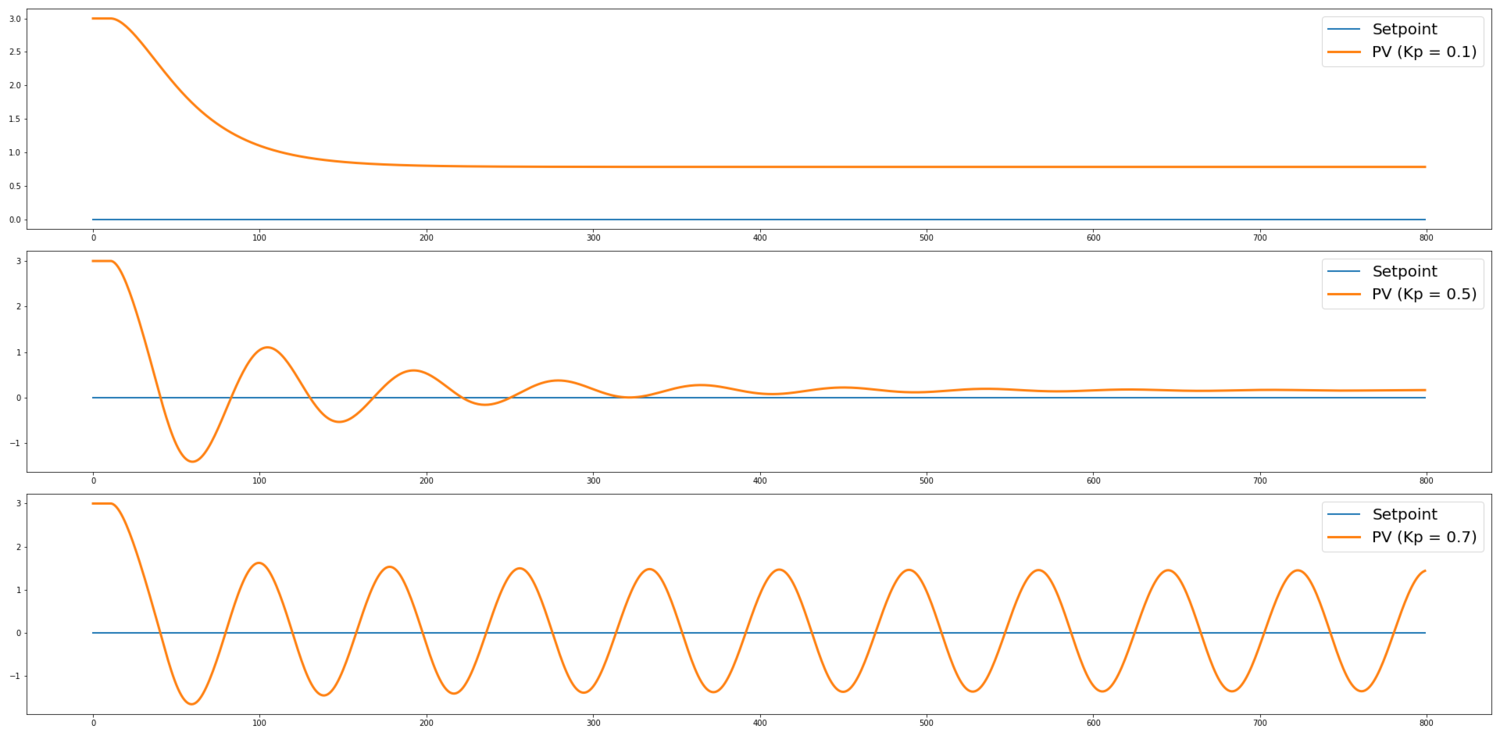
\includegraphics[width=0.666\textwidth]{proportional_control.png}
  \caption{Examples of different P Gain values}
\end{figure}
\noindent
However, only the Proportional Control alone is not enough since it does not eliminate the steady-state error (persistent offset) and also the time-consuming convergence to the setpoint.

\begin{figure}[H]
  \centering
  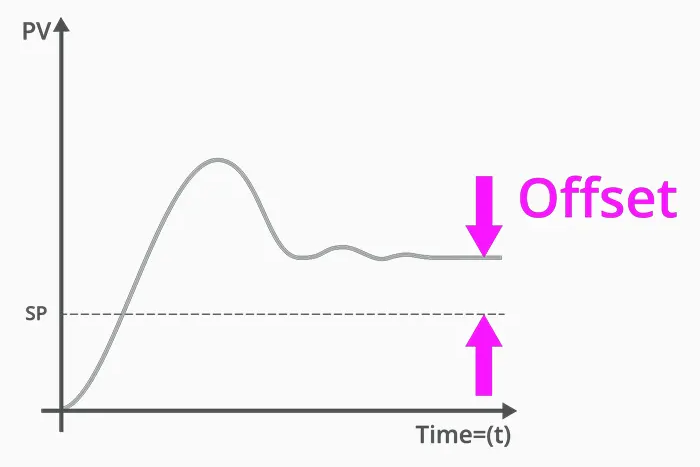
\includegraphics[width=0.5\textwidth]{offset.png}
  \caption{Steady-state Error}
\end{figure}

\subsubsection{Integral Control (I)}
To get rid of the steady-state error of the slow P-Controller, the integral term could be utilized to accumulate the error over time and therefore adjusts the control variable to the setpoint:
$$I = K_I\cdot\int_0^t e(t)dt$$
The incorrectly tuned Integral gain may results in under-damped (slow reaction) system or oscillating behavior.
The following image contains some examples of the behavior of the system if the Integral Gain is set too low, ideal and too high.
\begin{figure}[H]
  \centering
  \begin{subfigure}[b]{0.3\textwidth}
    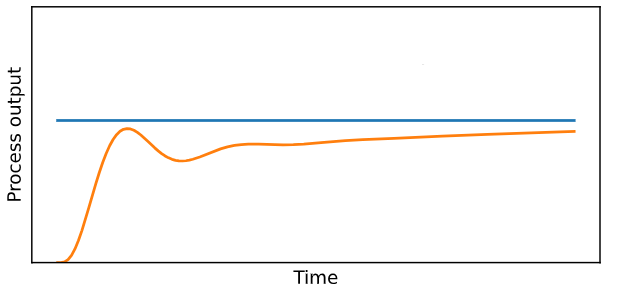
\includegraphics[width=\textwidth]{integral_low.png}
    \caption{I Gain too low}
  \end{subfigure}
  \hfill
  \begin{subfigure}[b]{0.3\textwidth}
    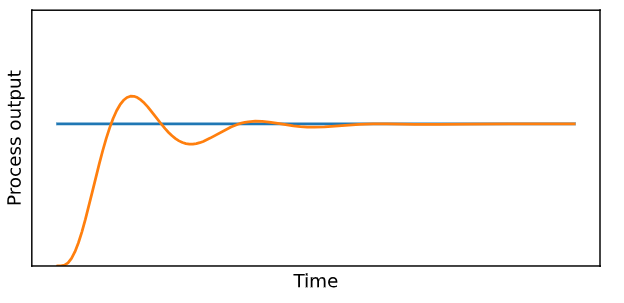
\includegraphics[width=\textwidth]{integral_ideal.png}
    \caption{I Gain ideal}
  \end{subfigure}
  \hfill
  \begin{subfigure}[b]{0.3\textwidth}
    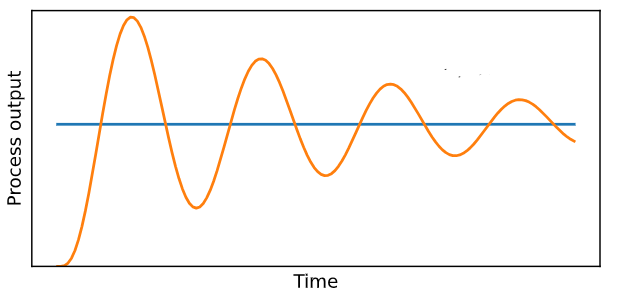
\includegraphics[width=\textwidth]{integral_high.png}
    \caption{I Gain too high}
  \end{subfigure}
  \caption{Examples of several values of I-Gain}
\end{figure}

\subsubsection{Derivative Control (D)}
The derivative term predicts future errors by considering the rate of error change.
$$D = K_D\cdot\frac{d e(t)}{dt}$$
Implementing this term will help increase the system damping effect since the rate of change (velocity) of the error is considered.
However, to high Derivative Gain may also lead to extensive overshoot of the system and noise is also a significant factor to be considered when tuning this constant.
\begin{figure}[H]
  \centering
  \begin{subfigure}[b]{0.3\textwidth}
    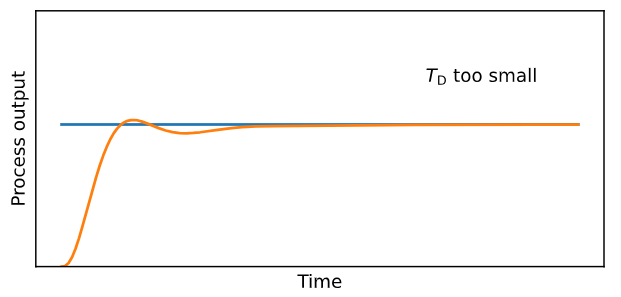
\includegraphics[width=\textwidth]{derivative_low.png}
    \caption{D Gain too low}
  \end{subfigure}
  \begin{subfigure}[b]{0.3\textwidth}
    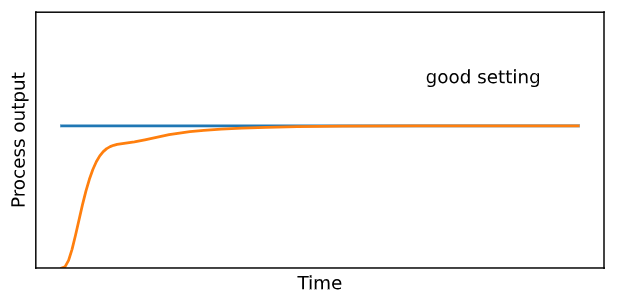
\includegraphics[width=\textwidth]{derivative_ideal.png}
    \caption{D Gain ideal}
  \end{subfigure}
  \begin{subfigure}[b]{0.3\textwidth}
    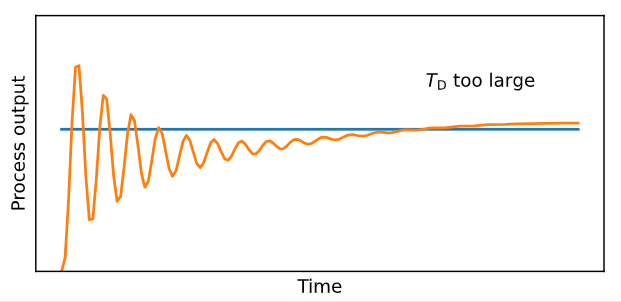
\includegraphics[width=\textwidth]{derivative_high.png}
    \caption{D Gain too high}
  \end{subfigure}
  \caption{Examples of several values of D-Gain}
\end{figure}

\subsubsection{Combined PID Control}
$$u(t) = K_P e(t) + K_I \int e(t) \, dt + K_D \frac{d e(t)}{dt}$$

\begin{wrapfigure}{l}{0.3\textwidth}
  \centering
  \addtolength{\belowcaptionskip}{-3ex}
  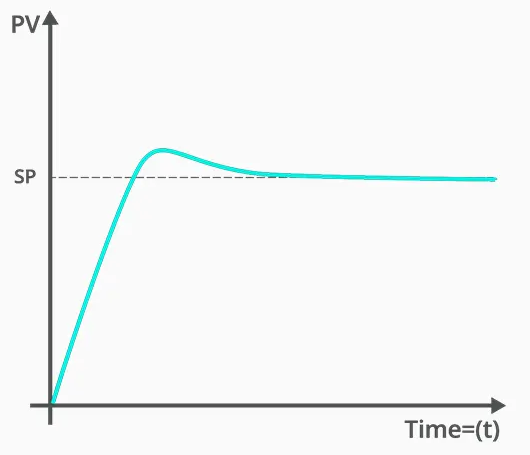
\includegraphics[width=0.3\textwidth]{full_pid.png}
  \caption{Combination of Proportional, Integral and Derivative controls}
\end{wrapfigure}

\noindent
In order to make the system behave robustly and perfectly, PID-tuning procedure must be conducted, in which of Proportional, Integral and Derivative Gains must be determined. Each parameter has different physical influence on the system, therefore it will be time-consumming to find the perfect conbination.

\subsection{Artificial Potential Field}
Artificial Potential Field is an approach to robot Path Planning problem that uses imaginary field generated on the robot's working environment, being a foundation for external Path Planning algorithms. The APF often consists of two types of force:
\begin{itemize}
  \item Attractive Force centered at the final desired position in robot's navigation acts as a directing tool.
  \item Repulsive Force placed along the edge of the obstacles helps repelling the robot when it gets close to the obstacle, providing the collision-free capability for the robot's navigation.
\end{itemize}
\begin{wrapfigure}{r}{0.4\textwidth}
  \centering
  \addtolength{\belowcaptionskip}{-0.8ex}
  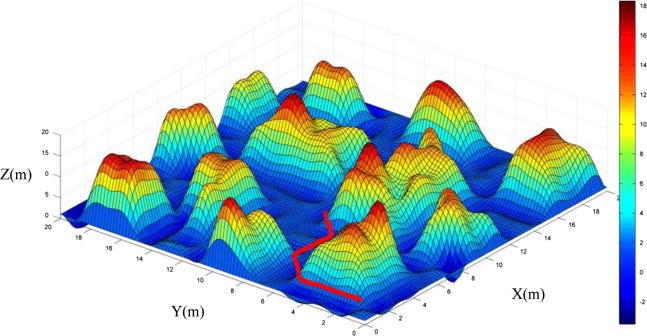
\includegraphics[width=0.4\textwidth]{apf_example.jpg}
  \caption{Artificial Potential Field}
\end{wrapfigure}

Another intuitive representation of the APF is by considering about the geographical meaning of it. Each of the obstacles can be assigned a "height", contributing to the total geographical terrain of the robot's working environment. The closer the vehicles gets to an obstacle, the steeper the slope it has to climb, the artificial gravitity will pull the vehicle down, hence, repelling it away from the mountain, or in this case, the obstacle. Through out this project, we will be using the geographic interpretation of APF as a supporting tool for the Genetic Algorithm introduced.

\subsection{Genetic Algorithm}
Genetic Algorithm is a heuristic adaptive search algorithm, part of the Evolutionary Algorithm which taken inspiration from the natural evolution of organisms. Genetic Algorithms iteratively modiy the genetic encoded chromosome of each individuals in a population with the principle of crossover and mutation, mimicking the evolution. The population then runs through a fitness function to be evaluated, or eliminated if its performance is too terrible.
\begin{figure}[H]
  \centering
  \begin{subfigure}[b]{0.45\textwidth}
    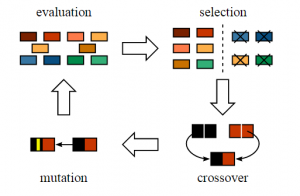
\includegraphics[width=\textwidth]{ga_example.png}
    \caption{Genetic Algorithm example}
  \end{subfigure}
  \begin{subfigure}[b]{0.45\textwidth}
    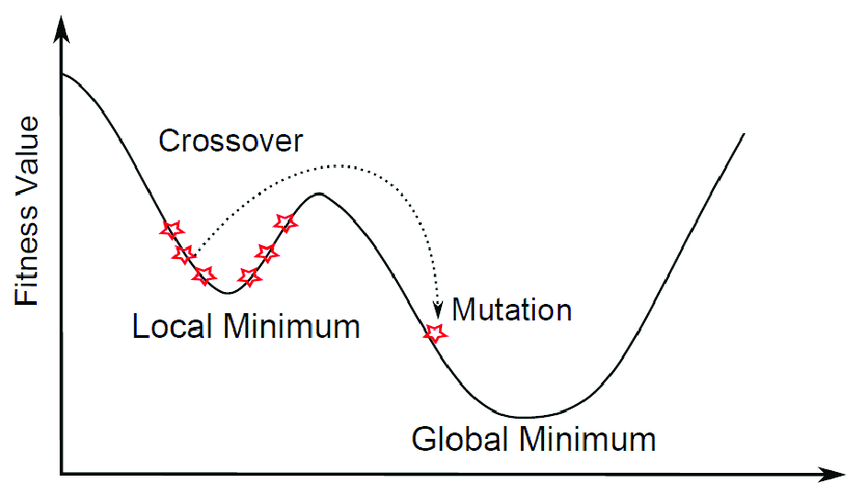
\includegraphics[width=\textwidth]{escaping_the_local_minima.png}
    \caption{Purpose of mutation}
  \end{subfigure}
  \caption{Some cases of Bézier Curve}
\end{figure}
\noindent
Relying on the natural selection principle, the chromosomes that yielded better performance (elites) will proceed to the next evolution, converging to an answer of the problem that we are trying to solve. Also, the randomness of natural mutation would provided the diversity of individuals that may produce better results, hence helping the model escape out of the local minima to find a better one.

\subsection{Gaussian Distribution}
\begin{wrapfigure}{r}{0.4\textwidth}
  \centering
  \addtolength{\belowcaptionskip}{-0.3ex}
  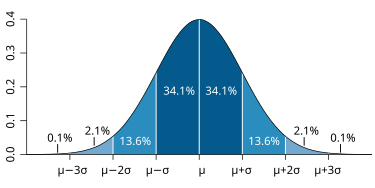
\includegraphics[width=0.35\textwidth]{gaussian_distribution.png}
  \caption{Gaussian Distribution}
\end{wrapfigure}

The Gaussian distribution, is a cornerstone of probability and statistics, distinguished by its symmetric, bell-shaped curve. Its prevalence in various natural process, which asserts that the aggregate of numerous independent random variables. This help the system to deal with the unexpectable real-life conditions.

\subsection{Binary Search Algorithm}
Binary Search Algorithm is a method of finding an element in a sorted array.
It does this by iteratively divide the array in half, looking for the element in either left and right partitions and ignore one them if the element lies on the other.
This is a very efficient algorithm in searching problems, especially for those with sorted values like ours because by repeatedly cutting the problem in half, the complexity is on the logarithmic scale.
\begin{figure}[H]
  \centering
  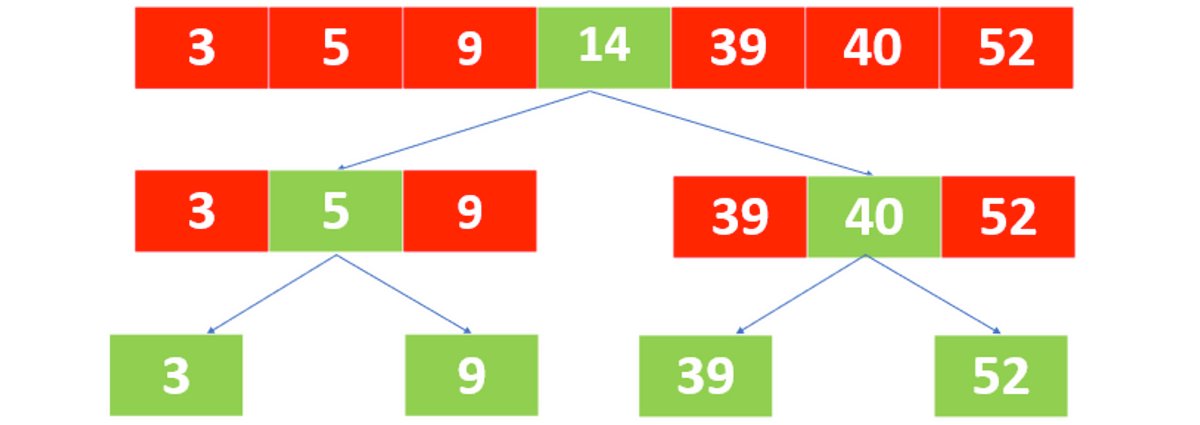
\includegraphics[width=0.55\textwidth]{binary_search.png}
  \caption{Binary Search Visualization}
\end{figure}
